%% LyX 2.3.2 created this file.  For more info, see http://www.lyx.org/.
%% Do not edit unless you really know what you are doing.
\documentclass[a4paper,english]{article}
\usepackage[T1]{fontenc}
\usepackage[latin9]{inputenc}
\usepackage{color}
\usepackage{amssymb}
\usepackage{graphicx}

\makeatletter

%%%%%%%%%%%%%%%%%%%%%%%%%%%%%% LyX specific LaTeX commands.
\special{papersize=\the\paperwidth,\the\paperheight}

%% Because html converters don't know tabularnewline
\providecommand{\tabularnewline}{\\}

%%%%%%%%%%%%%%%%%%%%%%%%%%%%%% User specified LaTeX commands.
%% use full paper
\usepackage[margin=2cm]{geometry}

%% multicols
\usepackage{multicol}

%% no automated date after title 
\date{}

%% compact spacing
\usepackage[compact]{titlesec}
\usepackage{enumitem}
\setlist{nolistsep}

%% table formatting
\usepackage{graphicx} 

%% colors
\usepackage{xcolor, amsmath}
\usepackage[linesnumbered,ruled,vlined]{algorithm2e}
\definecolor{amaranth}{rgb}{0.9, 0.17, 0.31}
\DontPrintSemicolon
% Define pseudocode formatting
\renewcommand{\KwSty}[1]{\textnormal{\textcolor{amaranth!90!black}{\bfseries #1}}\unskip}
\renewcommand{\ArgSty}[1]{\textnormal{\ttfamily #1}\unskip}
\SetKwComment{Comment}{\color{green!80!black!190}// }{}
\renewcommand{\CommentSty}[1]{\textnormal{\ttfamily\color{green!80!black!190}#1}\unskip}
\newcommand{\assign}{\leftarrow}
\newcommand{\var}{\texttt}
\newcommand{\FuncCall}[2]{\texttt{\bfseries #1(#2)}}
\SetKwProg{Function}{Function}{}{}
\SetKw{Continue}{continue}
\renewcommand{\ProgSty}[1]{\texttt{\bfseries #1}}
%\usepackage{etoolbox}
\usepackage{setspace}
%\AtBeginEnvironment{algorithm}{\setstretch{0.75}}


% text highlight
\newcommand{\hyellow}[1]{\colorbox{yellow!20}{#1}}
\newcommand{\horange}[1]{\colorbox{orange!20}{#1}}
\newcommand{\hgreen}[1]{\colorbox{green!20}{#1}}
\newcommand{\hred}[1]{\colorbox{red!20}{#1}}

% titlespace
\usepackage{titling}

% no ugly indent
\setlength\parindent{0pt}

% algorithm highlight
\usepackage{tikz}
\usetikzlibrary{fit,calc}
%define a marking command
\newcommand*{\tikzmk}[1]{\tikz[remember picture,overlay] \node (#1) {};\ignorespaces}
%define a boxing command, argument = colour of box
\newcommand{\boxit}[1]{\tikz[remember picture,overlay]{\node[yshift=3pt,fill=#1,opacity=.25,fit={(A)($(B)+(.5\linewidth,0.9\baselineskip)$)}] {};}\ignorespaces}

% define some colours according to algorithm parts (or any other method you like)
\colorlet{green}{green!30}
\colorlet{yellow}{yellow!20}
\colorlet{red}{red!20}

% algorithm comments on the right side
\usepackage{algpseudocode}

\makeatother

\usepackage{babel}
\usepackage{listings}
\lstset{frame=trbl,
backgroundcolor={\color{lightgray}},
flexiblecolumns=true,
basicstyle={\small\ttfamily},
breaklines=true,
keywordstyle={\color{blue}\bfseries},
language=Java,
sensitive=true,
emph={[1]{critical_section}},
emphstyle={[1]\color{red}},
emph={[2]{atomic,Condition}},
emphstyle={[2]\color{blue}},
rulesepcolor={\color{gray}},
emph={[3]{acquire(mutex),release(mutex),signal(mutex)}},
emphstyle={[3]\color{magenta}},
showstringspaces=false,
stringstyle={\color{purple}},
commentstyle={\usefont{T1}{pcr}{m}{sl}\color{MyDarkGreen}\small},
morecomment={[l][\color{Blue}]{...}},
tabsize=4,
lineskip={-1.5pt}}
\begin{document}
\title{C\texttt{++} DP-GBDT Side-channel Analysis}

\maketitle
\tableofcontents{}

\pagebreak{}

\section{Severity List}

\paragraph{General\protect \\
}

\begin{tabular}{|c|c|}
\hline 
entity & secrecy\tabularnewline
\hline 
\hline 
X & $\checkmark$\tabularnewline
\hline 
X\_cols\_size & $\times$\tabularnewline
\hline 
X\_rows\_size & $\times$\tabularnewline
\hline 
y & $\checkmark$\tabularnewline
\hline 
y\_rows\_size & $\times$\tabularnewline
\hline 
\end{tabular} ~~~%
\begin{tabular}{|c|c|}
\hline 
parameter & secret\tabularnewline
\hline 
\hline 
nb\_trees & $\times$\tabularnewline
\hline 
learning\_rate & $\times$\tabularnewline
\hline 
privacy\_budget & $\times$\tabularnewline
\hline 
task & $\times$\tabularnewline
\hline 
max\_depth & $\times$\tabularnewline
\hline 
min\_samples\_split & $\times$\tabularnewline
\hline 
balance\_partition & $\times$\tabularnewline
\hline 
gradient\_filtering & $\times$\tabularnewline
\hline 
leaf\_clipping & $\times$\tabularnewline
\hline 
scale\_y & $\times$\tabularnewline
\hline 
use\_decay & $\times$\tabularnewline
\hline 
l2\_threshold & $\times$\tabularnewline
\hline 
l2\_lambda & $\times$\tabularnewline
\hline 
cat\_idx & $\times$\tabularnewline
\hline 
num\_idx & $\times$\tabularnewline
\hline 
\end{tabular} ~~~%
\begin{tabular}{|c|c|}
\hline 
inferrable from those & secret\tabularnewline
\hline 
\hline 
nb\_samples per tree & $\times$\tabularnewline
\hline 
\end{tabular}

\paragraph{While building a single tree\protect \\
}

\begin{tabular}{|c|c|c|}
\hline 
entity & secrecy & \tabularnewline
\hline 
\hline 
X\_subset & $\checkmark$ & \tabularnewline
\hline 
X\_subset\_cols\_size & $\times$ & \tabularnewline
\hline 
X\_subset\_rows\_size & $\checkmark$ & \tabularnewline
\hline 
y\_subset & $\checkmark$ & \tabularnewline
\hline 
y\_subset\_rows\_size & $\checkmark$ & \tabularnewline
\hline 
gradients & $\checkmark$ & \tabularnewline
\hline 
gradients\_size & $\checkmark$ & \tabularnewline
\hline 
\end{tabular}

\pagebreak{}

\section{\texttt{main}}

\section{\texttt{class DPTree}}

\subsection{Creation / destruction / global variables}

\paragraph{Side channel leakage}

\subsection{Methods}

\subsubsection{\texttt{fit}}

\pagebreak{}

\subsubsection{\texttt{make\_tree\_DFS}}

\paragraph{Caller graph\protect \\
\protect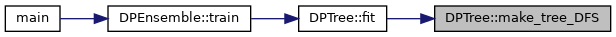
\includegraphics[scale=0.6]{/home/loretanr/ma/code/hardening/visualisation/graphs/make_tree_DFS/class_d_p_tree_a07314c44bb7b7ca37c735b70de3ccb9e_icgraph}}

\paragraph{Call graph\protect \\
\protect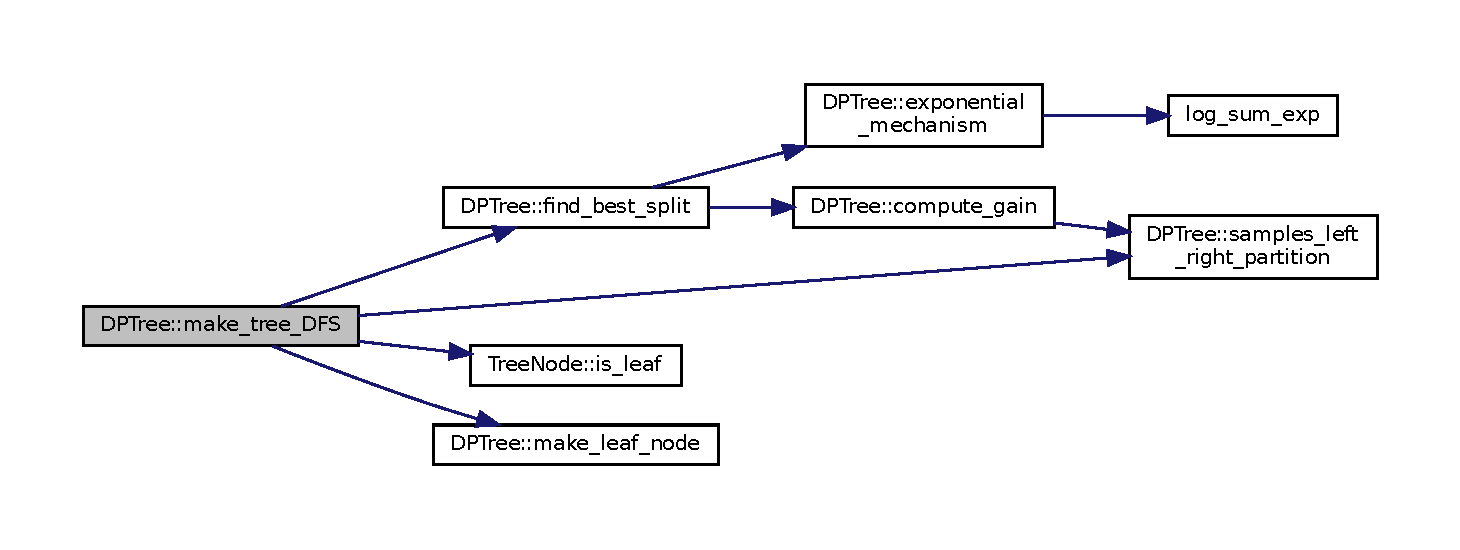
\includegraphics[scale=0.6]{/home/loretanr/ma/code/hardening/visualisation/graphs/make_tree_DFS/class_d_p_tree_a07314c44bb7b7ca37c735b70de3ccb9e_cgraph}}

\paragraph{Arguments / used variables\protect \\
}

\begin{multicols}{3}%
\begin{tabular}{|c|c|}
\hline 
variable & secret\tabularnewline
\hline 
\hline 
dataset & $\checkmark$\tabularnewline
\hline 
gradients & $\checkmark$\tabularnewline
\hline 
curr\_depth & ?\tabularnewline
\hline 
live\_samples & $\checkmark$\tabularnewline
\hline 
\end{tabular}

\begin{tabular}{|c|c|}
\hline 
params.min\_samples\_split & $\times$\tabularnewline
\hline 
params.max\_depth & $\times$\tabularnewline
\hline 
\end{tabular}

\end{multicols}

\begin{algorithm}\setstretch{0.9}
  \caption{make\_tree\_DFS}

  \Function{make\_tree\_DFS(live\_samples[], curr\_depth)}{

	\Comment{max depth reached or not enough samples -> leaf node}
    \If{curr\_depth == params.max\_depth || len(live\_samples) < params.min\_samples\_split}{
      	$\texttt{TreeNode *leaf = \emph{make\_leaf\_node(curr\_depth, live\_samples)}}$ \\
			\Return{$\texttt{leaf}$}\
    }

	\Comment{get actual sample rows and respective gradients from indices in live\_samples}
	$\texttt{X\_live = dataset\ensuremath{\rightarrow}X[live\_samples]}$ \\
	$\texttt{gradients\_live = dataset\ensuremath{\rightarrow}gradients[live\_samples]}$ \\
	
	\Comment{find best split}
	$\texttt{TreeNode *node = \emph{find\_best\_split(X\_live, gradients\_live, curr\_depth)}}$ \\
		
	\Comment{no split found}
    \If{node.is\_leaf }{
		\Return{$\texttt{node}$}\
    }

	\Comment{prepare the new live samples to continue recursion}
		$\var{lhs} = \texttt{\emph{samples\_left\_right\_partition(X\_live, node.feature\_index, node.feature\_value)}}$ \\
	\For{sample : live\_samples} {
		\If {lhs.contains(sample)} {
			$\texttt{lhs\_live\_samples.insert(sample)}$
		} \Else {
			$\texttt{rhs\_live\_samples.insert(sample)}$
		}
	}
	\Comment{recurse}
	$\texttt{node\ensuremath{\rightarrow}left = make\_tree\_DFS(lhs\_live\_samples, curr\_depth+1)}$ \\
	$\texttt{node\ensuremath{\rightarrow}right = make\_tree\_DFS(rhs\_live\_samples, curr\_depth+1)}$ \\
    \Return{$\texttt{node}$}\
  }
\end{algorithm}

\begin{multicols}{2}

\paragraph{Side channel leakage}
\begin{itemize}
\item leakage in called methods
\end{itemize}
From branches/loops:
\begin{itemize}
\item \hgreen{params.max\_depth}
\item \hgreen{params.min\_samples\_split}
\item \hyellow{curr\_depth == max\_depth}
\item \hgreen{number of features (columns of X)}
\item \hred{number of live samples resp. rows in X\_live}
\item \hred{whether node becomes a leaf / \#leaves}
\item \hred{whether split is done on a categorical feature}
\item \hred{split details (how many samples go left/right)}
\end{itemize}
Recursion leakage: ?
\begin{itemize}
\item \hred{e.g. \#splits in the tree by measuring time}
\item \hred{\#nodes observable by watching memory allocations for nodes}
\end{itemize}
\end{multicols}

\paragraph{Mitigations}

TODO

\newpage{}

\subsubsection{\texttt{exponential\_mechanism}}

TODO

\newpage{}

\subsubsection{\texttt{find\_best\_split}}

\paragraph{Caller graph\protect \\
\protect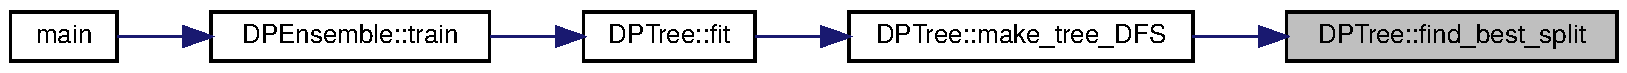
\includegraphics[scale=0.6]{../visualisation/graphs/find_best_split/caller}}

\paragraph{Call graph\protect \\
\protect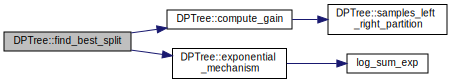
\includegraphics[scale=0.6]{../visualisation/graphs/find_best_split/call}}

\paragraph{Arguments / used variables\protect \\
}

\begin{multicols}{3}%
\begin{tabular}{|c|c|}
\hline 
variable & secret\tabularnewline
\hline 
\hline 
X & $\checkmark$\tabularnewline
\hline 
gradients & $\checkmark$\tabularnewline
\hline 
curr\_depth & ?\tabularnewline
\hline 
tree\_budget & $\times$\tabularnewline
\hline 
\end{tabular}

\begin{tabular}{|c|c|}
\hline 
params.use\_decay & $\times$\tabularnewline
\hline 
params.$\Delta g$ & $\times$\tabularnewline
\hline 
params.max\_depth & $\times$\tabularnewline
\hline 
\end{tabular}

\end{multicols}

\begin{algorithm}\setstretch{0.9}
  \caption{find\_best\_split}
  \Function{find\_best\_split(X[][], gradients[], curr\_depth)}{

	\tcp{determine node privacy budget}
	\tikzmk{A}
    \If(\algorithmiccomment{this is a comment}){params.use\_decay}{  
			\tikzmk{B}\boxit{green}\tikzmk{A}
      	\If(\algorithmiccomment{this is another comment}){curr\_depth == 0}{
      		$\var{node\_budget} = \frac{\var{tree\_budget}}{2*({2^{\var{max\_depth}+1}} + 2^{\var{curr\_depth}+1})}$
	    } \Else {
				$\var{node\_budget} = \frac{\var{tree\_budget}}{2*{2^{\var{curr\_depth}+1}}}$
		}

    }\tikzmk{B}\boxit{yellow}\tikzmk{A} \Else {
		$\var{node\_budget} = \frac{\var{tree\_budget}}{2*\var{max\_depth}}$
	}\tikzmk{B}\boxit{green}

	\tcp{iterate over all possible splits}
	\For{feature\_index : features} {
		\For{feature\_value : X[feature\_index]} {
			\If {"already encountered feature\_value"} {
				\Continue
			}
			$\var{gain} = \texttt{\emph{compute\_gain(X, gradients, feature\_index, feature\_value)}}$ \\
			\If {gain < 0} {
				\Continue
			}
			$\var{gain} = \frac{\var{node\_budget} * \var{gain}}{2 * \Delta g}$ \\
			$\var{candidates}\texttt{.insert(Candidate(feature\_index, feature\_value, gain))}$
		}
	}

	\tcp{choose a split using the exponential mechanism}
	$\var{index} = \texttt{\emph{exponential\_mechanism(candidates)}}$ \\
	\tcp{construct the node}
	$\texttt{TreeNode *node = new TreeNode(candidates[index])}$ \\
    \Return{$\texttt{node}$}\;
  }
\end{algorithm}

\paragraph{Side channel leakage}

\begin{multicols}{2}
\begin{itemize}
\item leakage in \texttt{compute\_gain} and \texttt{exponential\_mechanism}
\end{itemize}
From branches/loops:
\begin{itemize}
\item \hgreen{params.use\_decay}
\item \hyellow{curr\_depth == 0}
\item \hgreen{number of features (columns of X)}
\item \hred{number of rows in X resp. length of gradients}
\item \hred{number of unique feature values of a feature}
\item \hyellow{number of splits that don't give any gain}
\item \hyellow{number of split candidates}
\end{itemize}
Potential arithmetic leakage: ?
\begin{itemize}
\item Not sure about this in SGX though
\item edge cases of variables appearing in formulas $\rightarrow$ \texttt{tree\_budget}
and \texttt{curr\_depth} and $\Delta g$ and \texttt{gain}
\end{itemize}
\end{multicols}

\paragraph{Mitigations}

TODO

\pagebreak{}

\subsubsection{\texttt{compute\_gain}}

\paragraph{Caller graph\protect \\
\protect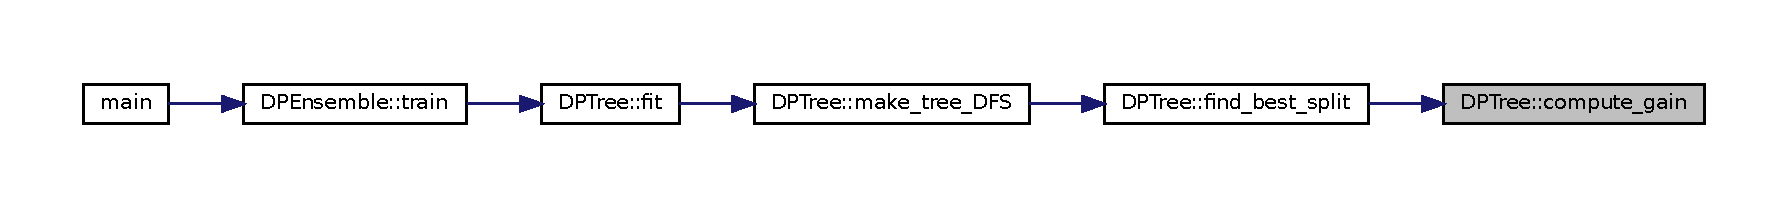
\includegraphics[scale=0.6]{/home/loretanr/ma/code/hardening/visualisation/graphs/compute_gain/class_d_p_tree_ab9426a6ac2e5122e29ecbb6e9c4cd050_icgraph}}

\paragraph{Call graph\protect \\
\protect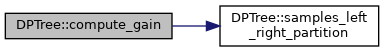
\includegraphics[scale=0.6]{/home/loretanr/ma/code/hardening/visualisation/graphs/compute_gain/class_d_p_tree_ab9426a6ac2e5122e29ecbb6e9c4cd050_cgraph}}

\paragraph{Arguments / used variables\protect \\
}

\begin{tabular}{|c|c|c|}
\hline 
variable & secret & \tabularnewline
\hline 
\hline 
X & $\checkmark$ & \tabularnewline
\hline 
gradients & $\checkmark$ & \tabularnewline
\hline 
feature\_index & $\times$ & \tabularnewline
\hline 
feature\_value & $\times$ & \tabularnewline
\hline 
params.l2\_lambda & $\times$ & \tabularnewline
\hline 
\end{tabular}

\begin{algorithm}\setstretch{0.9}
  \caption{compute\_gain}
  \Function{compute\_gain(X[][], gradients[], feature\_index, feature\_value)}{
	
	\Comment{// partition into lhs/rhs}
     $\var{lhs}, \var{rhs} = \texttt{\emph{samples\_left\_right\_partition(X, feature\_index, feature\_value)}}$ \\
		$\var{lhs\_size} = \texttt{lhs.size()}$ \\
		$\var{rhs\_size} = \texttt{rhs.size()}$

	\Comment{return on useless split}
	\If{lhs\_size == 0 || rhs\_size == 0} {
		\Return{$\texttt{-1}$}
	}
	\Comment{sums of lhs/rhs gains}
	$\var{lhs\_gain} = \texttt{sum(gradients[lhs])}$ \\
	$\var{rhs\_gain} = \texttt{sum(gradients[rhs])}$ \\
	$\var{lhs\_gain} = \frac{\var{lhs\_gain}^{2}}{\var{lhs\_size} + \var{params.l2\_lambda}}$ \\
	$\var{rhs\_gain} = \frac{\var{rhs\_gain}^{2}}{\var{rhs\_size} + \var{params.l2\_lambda}}$ \\
	$\var{total\_gain} = \var{lhs\_gain} + \var{rhs\_gain}$ \\
	$\var{total\_gain} = \texttt{max(total\_gain, 0)}$ \\

    \Return{$\texttt{total\_gain}$}\;
  }
\end{algorithm}

\paragraph{Side channel leakage}

\begin{multicols}{2}
\begin{itemize}
\item leakage in \texttt{samples\_left\_right\_partition}
\end{itemize}
From branches/loops/function calls:
\begin{itemize}
\item \hred{size (\#rows) of X/gradients}
\item \hred{lhs/rhs size}
\item \hyellow{whether it's a useless split}
\item \hred{memory access pattern of left/right gradients}
\item \hyellow{max function might leak whether \texttt{total\_gain} < 0}
\end{itemize}
Potential arithmetic leakage: ?
\begin{itemize}
\item edge cases of variables appearing in formulas $\rightarrow$ \texttt{lhs\_gain}
and \texttt{lhs\_size}, rhs respectively.
\end{itemize}
\end{multicols}

\paragraph{Mitigations}

TODO

\newpage{}

\subsubsection{\texttt{make\_leaf\_node}}

\subsubsection{\texttt{predict}}

\subsubsection{\texttt{samples\_left\_right\_partition}}

\subsubsection{\texttt{predict}}

\section{\texttt{class DPEnsemble}}

\subsection{Creation / destruction / global variables}

\paragraph{Side channel leakage}

\subsection{Methods}

\subsubsection{\texttt{train}}

\subsubsection{\texttt{predict}}

\subsubsection{\texttt{update\_gradients}}

\subsubsection{\texttt{add\_laplacian\_noise}}

\subsubsection{\texttt{remove\_rows}}

\subsubsection{\texttt{get\_subset}}

\section{other classes}
\end{document}
